\section{The Higgs Boson}

The Higgs boson is the only scalar particle present in the current formulation
of the SM. It is predicted to be massive with neither electric nor colour
charge. It couples to all massive particles, including itself, with coupling
strengths related to the mass of the particle. The coupling strength of the
Higgs boson to gauge bosons, $V$, is proportional to $m_{V}^2$. Similarly, the
Yukawa interactions between Higgs bosons and fermions are predicted to occur
with strengths proportional to the mass of the fermions, $m_f$. The detection of
the Higgs boson and confirmation of its properties (e.g.\ spin, intrinsic
parity, mass-dependent coupling strengths\todo{CP?}) would represent evidence
for the BEH mechanism and the Glashow--Salam--Weinberg model of the electroweak
interaction.

In 2012, almost half a century after the proposal of the
Glashow--Salam--Weinberg model, the Higgs boson was discovered by the
ATLAS~\cite{HIGG-2012-27} and CMS~\cite{CMS-HIG-12-028} collaborations at the
Large Hadron Collider with a mass of about \SI{125}{\GeV}. Since its discovery,
extensive measurements of its properties have been performed showing remarkable
agreement with the SM predictions. In 2022, the Higgs boson mass has been
measured with relative errors approaching \SI{0.1}{\percent}. An exemplary
measurement of the Higgs boson mass by the ATLAS collaboration yields
\begin{align*}
  m_{H} = \num{124.99}%
  \valuesep\numerrt{0.18}{stat.}%
  \valuesep\numerrt{0.04}{syst.}%
  \valuesep\si{\GeV}
\end{align*}
in the $H \to Z Z^{*} \to 4\ell$ channel~\cite{HIGG-2020-07} using \pp-collision
events collected during Run~2 of the Large Hadron Collider. The scalar nature of
the Higgs boson has been
confirmed~\cite{HIGG-2013-17-witherratum,CMS-HIG-14-018} and its coupling
strengths are thus far in good agreement with the SM
predictions~\cite{HIGG-2021-23,CMS-HIG-22-001}. As a result, the electroweak
sector is well established and the two parameters of the BEH potential, $v$ and
$m_{H}$, are measured with high precision.\footnote{The VEV was known prior to
  the discovery of the Higgs boson through measurements of the muon lifetime
  which allows to determine the effective coupling constant $G_{\text{F}}$ of
  the charged-current weak interaction. With known $G_{\text{F}}$, the VEV can
  be determined according to
  $v = \bigl( \sqrt{2} G_{\text{F}} \bigr)^{-1/2} \approx
  \SI{246}{\GeV}$~\cite{MuLan:2010shf}.}


\subsection{Production and Decay Modes}

The production of Higgs bosons at the LHC occur through different production
modes with production cross sections spanning multiple orders of magnitude. The
Feynman diagrams of the four dominant production modes are shown in
\Cref{fig:higgs_prod_feyn}, all of which have been experimentally confirmed. The
production cross section in \pp-collisions at a centre-of-mass energy of
\SI{13}{\TeV} is shown in \Cref{fig:higgs_prod_xsec} as a function of
$m_{H}$. For $m_{H} = \SI{125.0}{\GeV}$, the \ggF production mode has the
largest production cross section with
$\sigma(\pp \to H) \approx \SI{50}{\pico\barn}$, followed by the the VBF mode
with $\sigma(\pp \to qqH) \approx \SI{4}{\pico\barn}$, the $VH$ mode with
$\sigma(\pp \to VH) \approx \SI{2}{\pico\barn}$ inclusive in $V = W^\pm$ and
$V= Z$, and finally the $\ttbar H$ mode with
$\sigma(\pp \to \ttbar H) \approx
\SI{0.5}{\pico\barn}$~\cite{deFlorian:2016spz}. Higgs boson production modes
involving two Higgs bosons in the final state, which are the processes of
primary interest for this thesis, are covered in
\Cref{fig:theory_higgs_pair_prod}.

\begin{figure}[htbp]
  \centering

  \begin{subfigure}{0.48\textwidth}
    \centering
    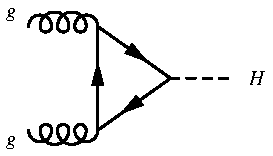
\includegraphics[scale=1]{feynman_graphs/higgs_prod_ggf}
    \subcaption{Gluon-gluon fusion (\ggF)}
  \end{subfigure}%
  \begin{subfigure}{0.48\textwidth}
    \centering
    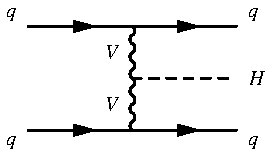
\includegraphics[scale=1]{feynman_graphs/higgs_prod_vbf}
    \subcaption{Vector boson fusion (VBF)}
  \end{subfigure}

  \vspace*{0.5em}

  \begin{subfigure}{0.48\textwidth}
    \centering
    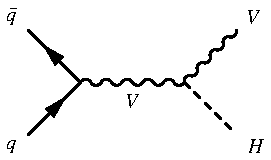
\includegraphics[scale=1]{feynman_graphs/higgs_prod_vh}
    \subcaption{Associated production with a massive vector boson ($VH$)}
  \end{subfigure}%
  \begin{subfigure}{0.48\textwidth}
    \centering
    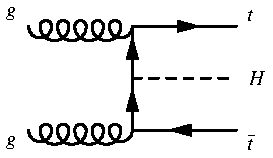
\includegraphics[scale=1]{feynman_graphs/higgs_prod_tth}
    \subcaption{Associated production with \ttbar ($\ttbar H$)}
  \end{subfigure}%

  \caption{The dominant Higgs boson production modes in \pp-collisions at
    centre-of-mass energies of \SI{13}{\TeV}.}%
  \label{fig:higgs_prod_feyn}
\end{figure}

\begin{figure}[htbp]
  \centering

  \begin{subfigure}[b]{0.47\textwidth}
    \centering

    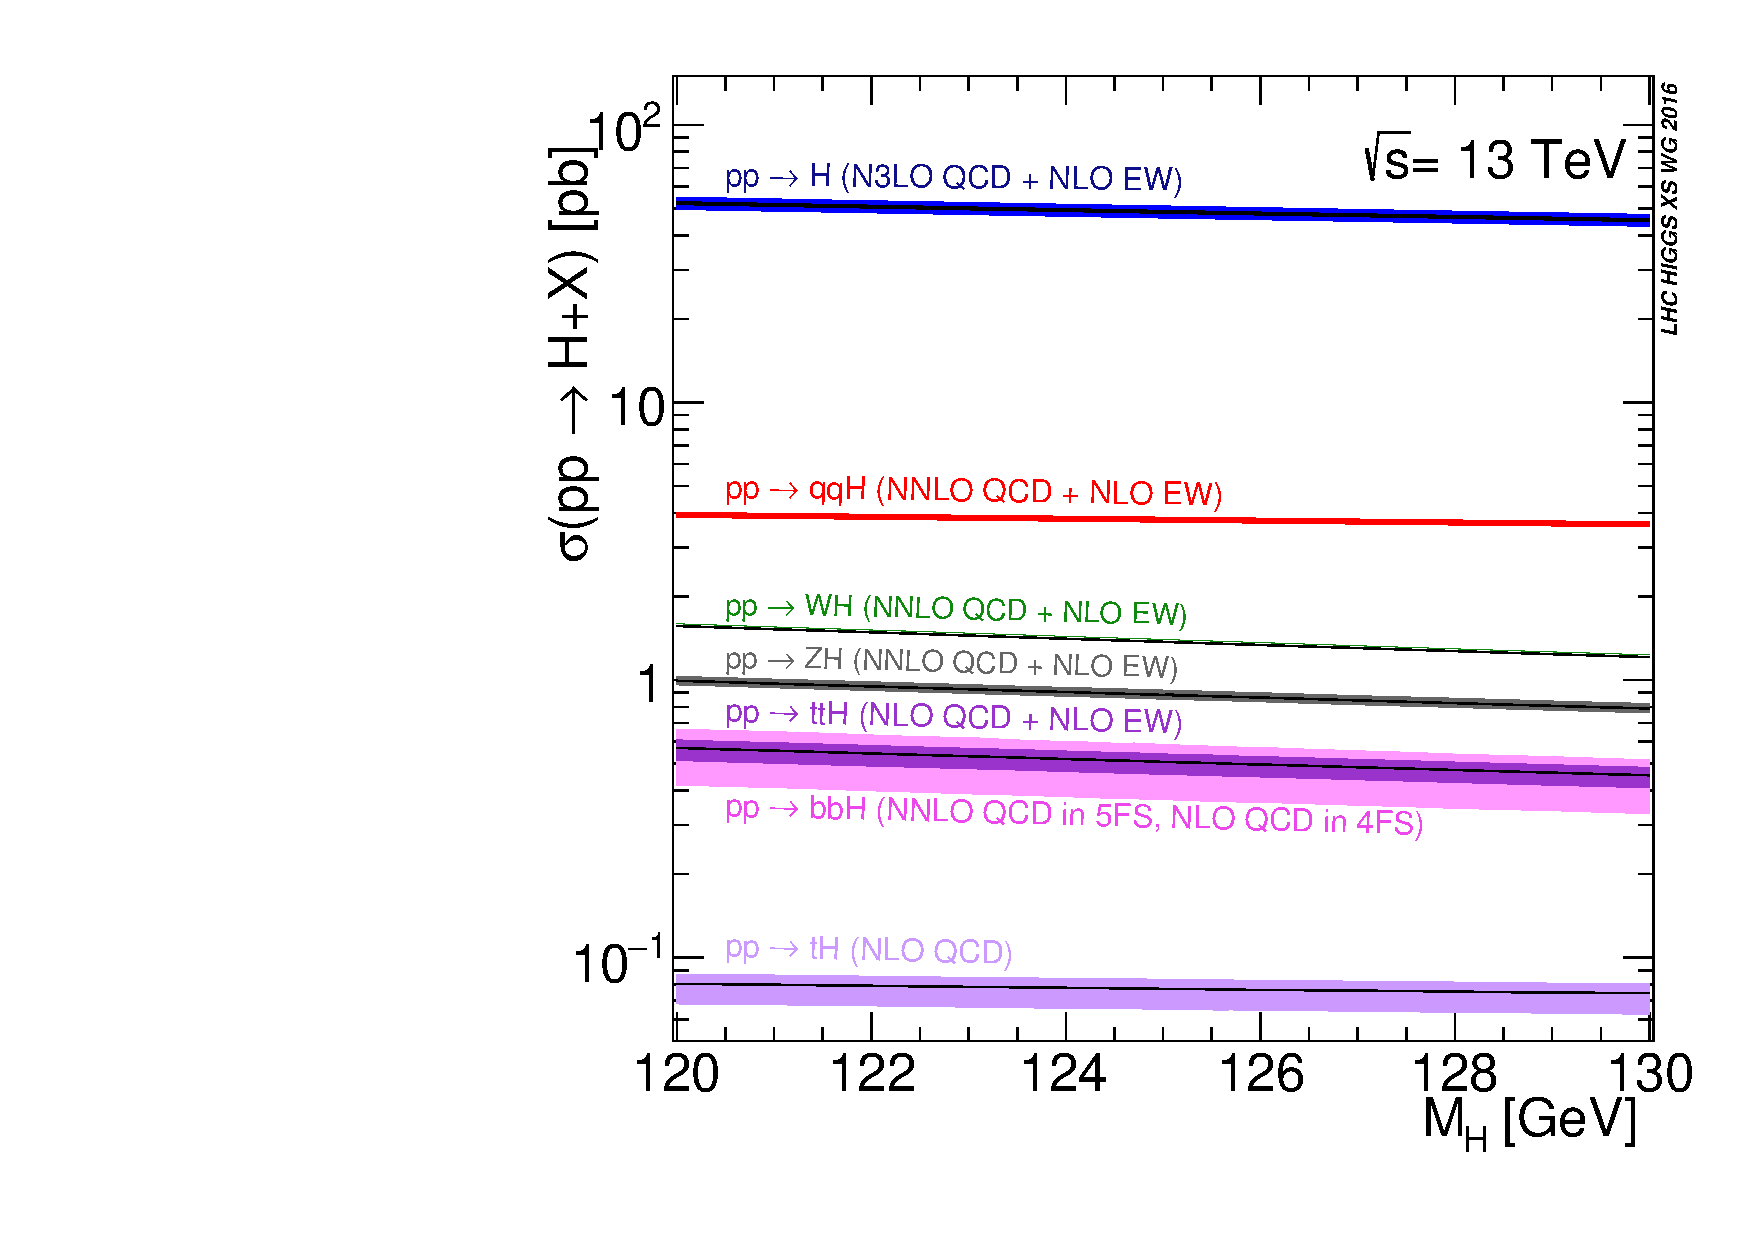
\includegraphics[width=0.95\textwidth]{theory/h_prod_crossec_13tev}

    \subcaption{Cross sections of Higgs boson production modes as a function of
      $m_{H}$.}%
    \label{fig:higgs_prod_xsec}
  \end{subfigure}\hfill%
  \begin{subfigure}[b]{0.47\textwidth}
    \centering

    \renewcommand{\arraystretch}{1.1}%
    \begin{tabular}{lS[table-format=2.3]c}
  \toprule
  Decay mode  & {BR / \%} & Observed \\
  \midrule
  $\bbbar$        & 58    & \checkmark \\
  $W^{+} W^{-}$    & 21    & \checkmark \\
  $gg$            & 8.2   & \\
  $\tau^+ \tau^-$ & 6.3   & \checkmark \\
  $c\bar{c}$      & 2.9   & \\
  $ZZ^{*}$            & 2.6   & \checkmark \\
  $\gamma\gamma$  & 0.23  & \checkmark \\
  $Z\gamma$       & 0.15  & \\
  $\mu^{+}\mu^{-}$ & 0.022 & $\sim$~\cite{CMS-HIG-19-006} \\
  \bottomrule
\end{tabular}

%%% Local Variables:
%%% mode: latex
%%% TeX-master: "../phd_thesis"
%%% End:


    \vspace*{1.2em}

    \subcaption{Branching ratios of Higgs boson decay modes. The $gg$,
      $\gamma\gamma$, and $Z\gamma$ decay modes occur via higher-order
      processes.}%
    \label{tab:higgs_branching_ratios}
  \end{subfigure}

  \caption{Higgs boson production cross section in \pp-collisions at a
    centre-of-mass energy of \SI{13}{\TeV} (a) and Higgs boson decay branching
    ratios for $m_{H} = \SI{125.0}{\GeV}$ (b). The figure and branching ratios
    are taken from Ref.~\cite{deFlorian:2016spz}.}
\end{figure}

The Higgs boson ($m_{H} = \SI{125}{\GeV}$) is predicted to have a total decay
width of about \SI{4}{\MeV}~\cite{deFlorian:2016spz} yielding a proper lifetime
of $10^{-22}\,\si{\second}$. As a result, the Higgs boson decays almost
immediately via one of the decay modes summarised in
\Cref{tab:higgs_branching_ratios} allowing detection only via its decay
products. The table reflects the preferential coupling of the Higgs boson to
heavy particles such as the weak gauge bosons\footnote{The decays of Higgs
  bosons to $W^+W^-$ and $ZZ$ are suppressed since $m_{H} < 2 m_{W} < 2 m_{Z}$
  such that one of the gauge bosons has to be produced \emph{off shell}.} and
third generation fermions. The vast majority of Higgs bosons decay into \bbbar
with a branching ratio of \SI{58}{\percent}. The $b$-quark is the heaviest
fermion that can be produced in decays of Higgs bosons with
$m_H = \SI{125}{\GeV}$, decays to top-quark pairs being forbidden due to
$m_t > m_H$. The second largest branching ratio to fermions is the decay
$H \to \tau^+ \tau^-$ with \SI{6.3}{\percent} due to the large mass of the
\taulepton of \SI{1.777}{\GeV}~\cite{pdg2020}. In addition, a first indication
of SM-like Yukawa coupling to fermions of the second generation exist in the
form of evidence for the process $H \to \mu^+ \mu^-$ by the CMS
collaboration~\cite{CMS-HIG-19-006}.


\subsection{Higgs Boson Pair Production}
\label{fig:theory_higgs_pair_prod}

Directly access the shape of the BEH potential.

Production cross sections assuming $m_{H} = \SI{125.0}{\GeV}$:
\begin{itemize}
\item \ggF: \SI{31.05}{\femto\barn}~\cite{Grazzini:2018bsd}
\item VBF: \SI{1.726}{\femto\barn}~\cite{Dreyer:2018qbw,LHCHWGHH}
\item Higgs boson pair production in association with \ttbar (Third largest
  $\ttbar HH$: \SI{0.775}{})
\end{itemize}
Factor 1000 smaller than single Higgs boson production

\begin{figure}[htbp]
  \centering

  \begin{subfigure}{0.49\textwidth}
    \centering
    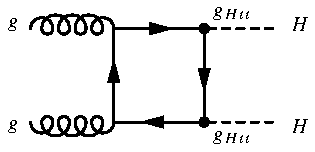
\includegraphics[width=0.7\textwidth]{feynman_graphs/di_higgs_box}
    \subcaption{}
  \end{subfigure}\hfill%
  \begin{subfigure}{0.49\textwidth}
    \centering
    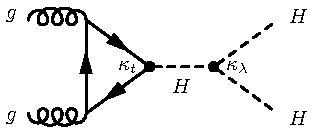
\includegraphics[width=0.7\textwidth]{feynman_graphs/di_higgs_triangle}
    \subcaption{}
  \end{subfigure}

  \vspace*{1em}

  \begin{subfigure}{0.33\textwidth}
    \centering
    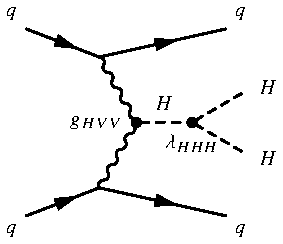
\includegraphics[width=0.95\textwidth]{feynman_graphs/di_higgs_vbf_kvklam}
    \subcaption{}
  \end{subfigure}\hfill%
  \begin{subfigure}{0.33\textwidth}
    \centering
    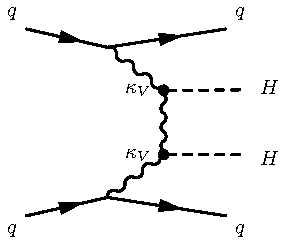
\includegraphics[width=0.95\textwidth]{feynman_graphs/di_higgs_vbf_kvkv}
    \subcaption{}
  \end{subfigure}\hfill%
  \begin{subfigure}{0.33\textwidth}
    \centering
    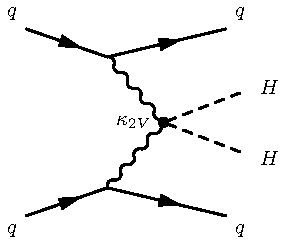
\includegraphics[width=0.95\textwidth]{feynman_graphs/di_higgs_vbf_ktwov}
    \subcaption{}
  \end{subfigure}

  \caption{Feynman diagrams of the two dominant production modes of Higgs boson
    pairs in \pp-collisions at centre-of-mass energies of \SI{13}{\TeV}.  The
    diagrams of the \ggF and VBF production mode are shown in (a-b) and (c-e),
    respectively.}%
  \label{fig:hh_feynmans}
\end{figure}



\begin{figure}[htbp]
  \centering
  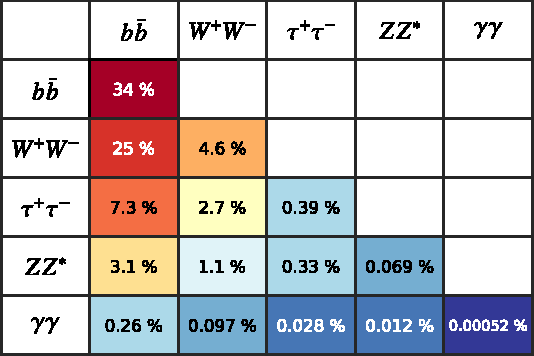
\includegraphics[width=0.45\textwidth]{theory/di_higgs_branching_ratio}
  \caption{Possible final states of decays of pairs of Standard Model Higgs
    bosons. Higgs boson branching ratios are taken from~\cite{deFlorian:2016spz}
    and assume~$m_{H} = \SI{125.0}{\GeV}$. The decay mode~$H \ra g g$ is
    excluded due to limited experimental feasibility.}
  \label{fig:hh_branching_ratios}
\end{figure}



\clearpage
\todo[inline]{Here be dragons}


\subsection{Higgs Boson Self-Interaction and Higgs Boson Pair Production}

Couplings of the Higgs boson to heavy vector bosons and heavy fermions
are quickly established after the Higgs boson discovery. However, the
Higgs boson self-coupling is still an open question and an important
probe to check EWSB.

% Super excellent talk by Katharine:
% https://indico.cern.ch/event/1065153/attachments/2351166/4011032/Seminar.pdf

All wrong...

Taylor expansion of the Higgs potential about the minimum after EWSB:
\begin{align*}
  V(h) &= \frac{1}{2} m_{\PH}^2 h^2 + \lambda v h^3 + \frac{1}{4} \lambda h^4 + \dots \\
  m_{\PH} &= \sqrt{2 \lambda v} \approx \SI{125}{\GeV} \\
  \lambda &\approx 0.13 \quad \text{(SM)}
\end{align*}
$h$ is a complex field with the $h^2$-term being the mass term,
$h^3$-term yielding the trilinear coupling, and the $h^4$-term
yielding the quartic coupling. All these terms are directly predicted
by the SM but an experimental probe is still justified to detect
possible deviations from the SM. The self-coupling strength~$\lambda$
can be directly probed in either double Higgs boson production or
triple Higgs boson production (although inaccessible
currently). Indirect probes also exist for example in single Higgs
boson production where the self-coupling contributes at loop-level.

Cross section of HH production is 1000 times smaller than single
Higgs. \todo{Cross section diagram would be nice?}

The Higgs potential in the SM is determined by two parameters:
$v = 1 / \sqrt{\sqrt{2} G_{\text{F}}^0}$ and $\lambda$



4b: Very large branching ratio but huge multi-jet background.

bbtautau: Can suppress multi-jet background reasonably but large
backgrounds from EW and top.

bbyy: Very clean, but low BR.

Sensitivity vs mass:

bbyy: Low mass sensitivity (due to low threshold photon triggers)

bbtautau: Medium mass sensitivity

bbbb: High mass sensitivity (BR and reduced problems in finding Higgs
candidates due to boost)

\todo[inline]{Experimental evidence for the top Yukawa coupling exists
  therefore non-resonant \HH production has to exist too (at least via
  the box diagram)}

\begin{description}


\item[Vacuum Stability] The present minimum with a vacuum expectation
  value of $v \approx \si{246}{\GeV}$ might be either a global minimum
  in which case the universe is stable or only a local minimum which
  leads to a metastable universe. In the metastable case, the state of
  the Higgs field could tunnel to a new local or global minimum with a
  smaller vacuum expectation value. Current experimental data cannot
  distinguish whether the universe is stable or
  meta-stable\todo{citation}.

\item[Elektroweak phase transition] In baryogenesis a first order
  electroweak phase transition is needed.

\item[BSM] Radions, 2HDM, Warped extra dimensions, composite Higgs,
  hMSSM, KK Gravitons: Most could decay to pairs of SM Higgs bosons.

\end{description}

Single Higgs boson production cross section
$\approx \SI{50}{\pico\barn}$. Compared to Higgs pair production cross
section $\approx \SI{30}{\femto\barn}$.

\todo[inline]{Shortcomings of the SM: Hierarchy problem, dark matter, quantum
  description of gravity}

\todo[inline]{Maybe: SUSY - superpartners - cancellation of loop corrections to $h$
  mass; In R-parity conserving SUSY - LSP - DM candidate}

\todo[inline]{What models predict Spin-0 resonances decaying into pair of SM
  Higgs? 2HDM}

\todo[inline]{Mention Spin-2 resonances? KK-graviton -- theoretically not favoured}

\todo[inline]{Scalar sector relatively unexplored?}

%%% Local Variables:
%%% mode: latex
%%% TeX-master: "../../phd_thesis"
%%% End:
